
This section details an example integration of the \COP with
the open source PicoRV32 RISC-V core.

The example integration consists of a single PicoRV32 and \COP
connected via the Pico Co-Processor Interface (PCPI).

The PCPI is a feature of the PicoRV32.
We include the glue logic required in order to interface with the \COP.

The resulting sub-system has two memory ports, one for the \COP and one
for the PicoRV32.
Both memory ports are configured as AXI4-Lite interfaces.

\subsection{Sub-System Overview}

Figure \ref{fig:integration-block} shows the main ports and connections in
the example integration.

\begin{figure}[h]
\centering
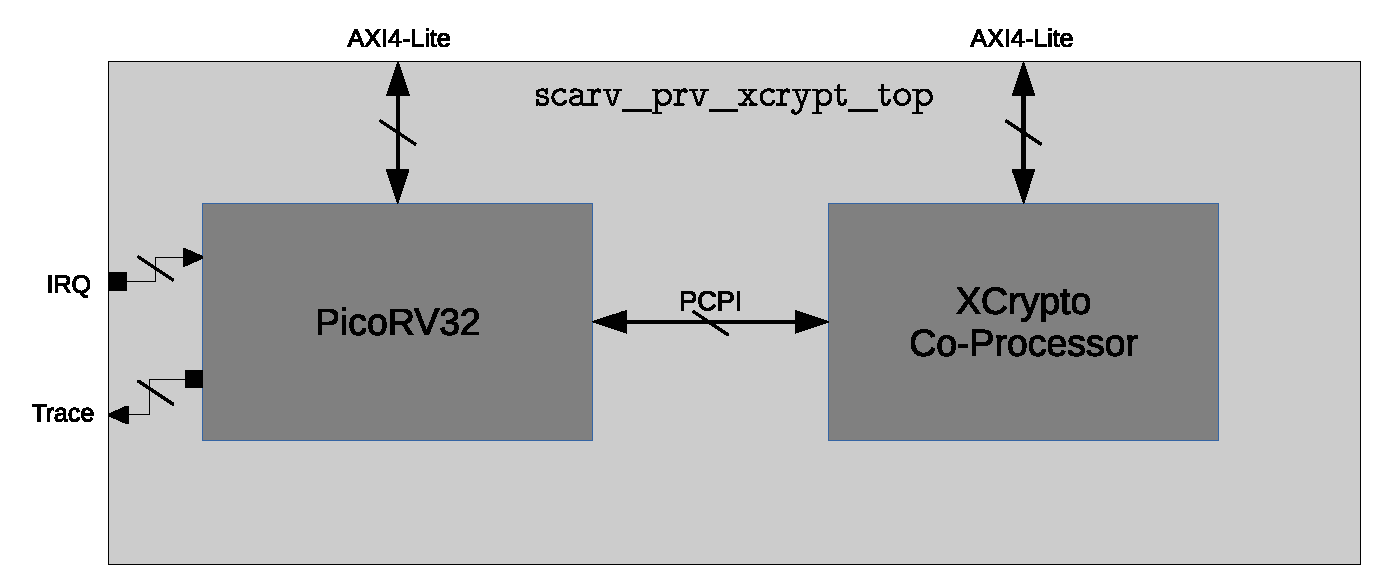
\includegraphics[width=1.0\textwidth]{diagrams/integration-block-diagram.eps}
\caption{Block diagram of the example \COP integration with the PicoRV32}
\label{fig:integration-block}
\end{figure}

The PicoRV32 memory, trace and interrupt interfaces are all exposed, along
with the \COP memory interface.

The top level module for the sub-system is {\tt scarv\_prv\_xcrypt\_top}.


\subsection{Integration Files}

This section lists the files required for working with the example
integration.

\subsubsection{Integration RTL}

The synthesisable RTL for the example integration is split across three
directories:

\begin{enumerate}
\item {\tt \$XC\_HOME/rtl/coprocessor} Contains all of the RTL dedicated
    to the \COP.
    This RTL will be required to create other custom integrations.
\item {\tt \$XC\_HOME/rtl/integration} Contains all of the RTL dedicated
    to the integration.
    Principally, it contains the glue logic for the
    sub-system top level, and the PCPI to \COP interface converter.
\item {\tt \$XC\_HOME/external/picorv32/} Contains the {\tt picorv32.v}
    file, which has all of the logic for the PicoRV32 core in it.
\end{enumerate}

\subsubsection{Integration Testbench}

All files for the integration testbench are found in 
{\tt \$XC\_HOME/verif/tb}.

The {\tt tb\_integration.v} file is the top-level testbench for the 
subsystem.
The {\tt axi\_sram.v} file contains simple AXI SRAM models used to simulate
a wider SoC.

Several "plusarg" options can be passed to the top level integration
testbench:

\begin{table}[h]
\begin{tabularx}{\textwidth}{l l Y}
\toprule
\textbf{Name} & \textbf{Type} & \textbf{Description} \\ \midrule
  IMEM        & String        & Memory hex file image to load. \\
  WAVES       & String        & Where to dump VCD waves file.  \\
  TIMEOUT     & Integer       & Number of clock cycles to simulate for. \\
  PASS\_ADDR  & Integer       & If the PicoRV32 requests this address, the 
    simulation will stop and report "SIM PASSED"    \\
  FAIL\_ADDR  & Integer       & If the PicoRV32 requests this address, the
    simulation will stop and report "SIM FAILED" \\
\bottomrule
\end{tabularx}
\end{table}

All of these plusargs are automatically filled by the simulation flow
when running {\tt make}.
By default, VCD waveforms will be dumped to
{\tt \$XC\_WORK/icarus/integ-waves.vcd}.
This can be overridden by exporting the environment variable
{\tt RTL\_WAVES} with the desired value.

Likewise, an arbitrary memory image can be specified using the
{\tt SIM\_UNIT\_TEST} environment variable.


\subsection{Integration Flow}

This section describes how to simulate and synthesise the example
integration sub-system.

\subsubsection{Simulation}

Building the integration testbench is done with:
\begin{lstlisting}[language=bash]  
$> make icarus_integ_tb
\end{lstlisting}

Running the integration testbench is done with:

\begin{lstlisting}[language=bash]
$> make icarus_run_integ
\end{lstlisting}

A specific memory image can be specified with:

\begin{lstlisting}[language=bash]
$> make icarus_run_integ SIM_UNIT_TEST=<path to .hex file>
\end{lstlisting}

Running {\tt make examples} will build a set of example programs which can
be easily run within the integration testbench.

Note that all tests under {\tt \$XC\_HOME/verif/unit} {\em can} be run
under the integration testbench, but they will fail out immediately
as they are designed to be run with the functional verification testbench.

\subsubsection{Synthesis}

The example synthesis flow uses {\tt yosys} to create a verilog netlist of
the combined CPU and co-processor.
The {\tt scarv\_prv\_xcrypt\_top} module is the top-level entity.

\begin{lstlisting}[language=bash]
$> make yosys_synth
\end{lstlisting}

\noindent
Will create the netlist and put the result in 
{\tt \$XC\_HOME/work/scarv\_cop\_top.v}.

\noindent
Extra report files include:
\begin{itemize}
\item {\tt \$XC\_HOME/work/yosys-synth.log} - 
    The log file for the synthesis process.
\item {\tt \$XC\_HOME/work/synth-statistics.rpt} - 
    The number of yosys internal cells used to represent the design.
    This is useful to work out the relative impact on area of different
    changes, though designers must be mindful this does not represent
    final FPGA utilisation or ASIC cell usage.
\item {\tt \$XC\_HOME/work/logic-loops.rpt} - 
    Contains reports on any logic loops found during the synthesis process.
    These must be removed before synthesis will complete.
\end{itemize}

\noindent
The {\tt yosys} script used is very simple, and is found in
{\tt \$XC\_HOME/flow/yosys/write-verilog.ys}.
